%after finding requirements more research is needed.
% Nummer, Vraag, label
\newcommand{\subquestion}[3]{
    \vspace{5mm}
    \noindent
    \textbf{Sub-question #1:} \emph{``#2''}
    \label{sq:Sub_question_#1#3}
    \newline
}
\section{Smart Home}
Main question: How does a smart home work?

\subsection{Hypothesis}
It is expected that the smart home will have multiple point of data, it centralises the data in an easy to read context so people can read the data. Data that will be found include: 
\begin{itemize}
    \item Power data of the power used in the home.
    \item Security information
    \begin{itemize}
        \item Camera images
        \item Locks
        \item Alarms
    \end{itemize}
    \item Temperature information
\end{itemize}
It will also be able to control the different equipment that is used in the house. These include:
\begin{itemize}
    \item The temperature
    \item When the lights will go on or off
    \item Timing certain uses of equipment like a dishwasher
\end{itemize}

\subsection{Sub-questions}
\begin{enumerate}
    \item What is a smart home?
    \item What are different types of smart homes?
    \item What kind of data does the smart home receive?
    \item What kind of data can the smart home control?
    \item How can the smart home be controlled?
\end{enumerate}

\subsection{Methodology}
To answer the main question the sub-questions need to be answered. To answer the sub-question it is important to explain the methods used. The methods are given below.\\
\subquestion{1}{What is a smart home?}{1}
In this chapter there will be different takes on what it means to have a smart home. It is necessary tat a look is taken at multiple research papers as to make a conclusion\\\\
\subquestion{2}{What are different types of smart homes?}{1}
To research this question smart home parts will be researched and the way it is used.\\\\
\subquestion{3}{What kind of data does the smart home receive?}{1}
This will be researched by reading papers of the possibilities and what had already been found.\\\\
\subquestion{4}{What kind of data can the smart home control?}{1}
This will be researched the same way as sub-question 2.\\\\
\subquestion{5}{How can the smart home be controlled?}{1}

\subsection{What is a smart home?}
In a research\cite{SmartHomecompare} that gives an overview of smart homes it states that:\textit{Smart home system offers people to control home environment in efficient and comfortable manner}. Another paper\cite{SmartHome_review} states that: \textit{Smart Home domain is a new trendy way of home automation and energy conservation}. A research paper\cite{SmartHomeTech} talking about the concept of the smart home states:\textit{Smart homes incorporate
common devices that control features of the home}, and that previously it was only used for environmental systems. With these three different papers it can be concluded that a smart home is a home that incorporates all common devices and control features.

\begin{figure}[H]
    \centering
    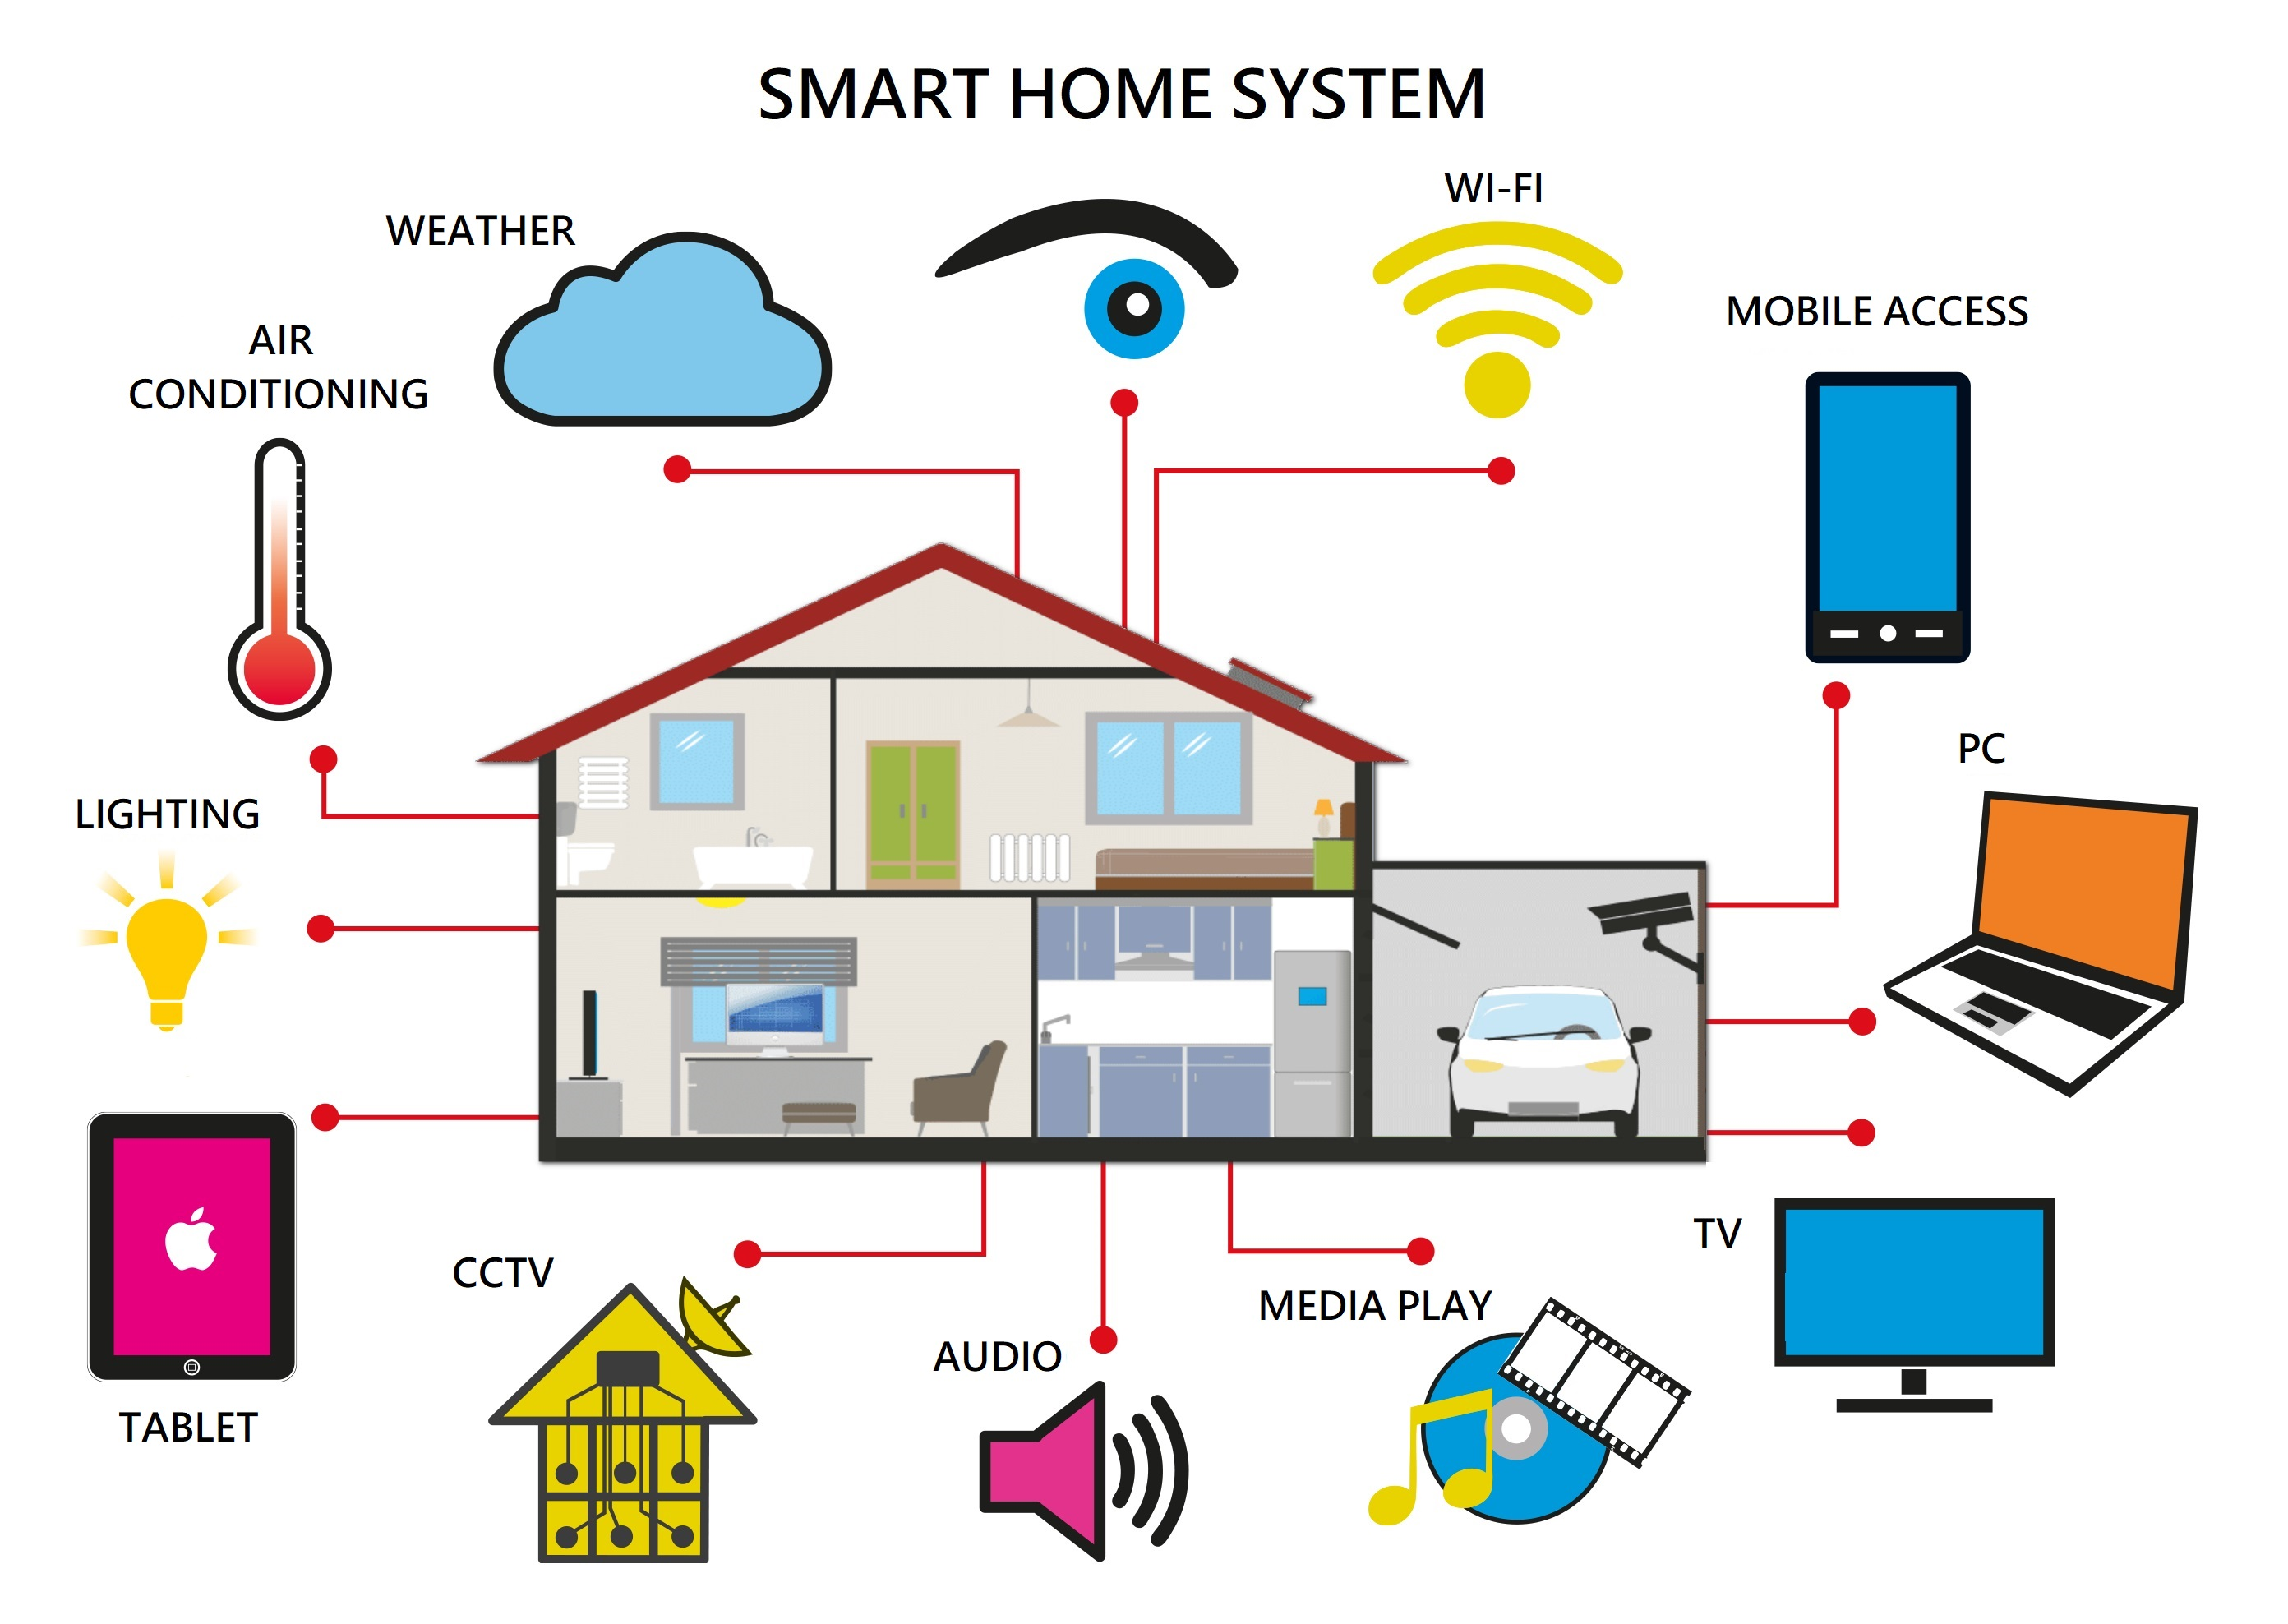
\includegraphics[width=10cm]{Images/Research/smart-home-01.jpg}
    \caption{Smart home}
    \label{fig:Smart_home}
\end{figure}

\subsection{Different types}
In a research\cite{SmartHomecompare} that compares and gives an overview of smart homes it states that there are different types of smart homes:
\begin{itemize}
    \item Dual tone multi frequency based(DTSM)
    \item Global system for mobile based(GSM)
    \item Voice recognition based
    \item Zigbee based
    \item Bluetooth based
    \item Internet and WiFi based
    \item Gesture based
\end{itemize}
The Zigbee, Bluetooth and internet and WiFi based types are all types that depend on the communication types. This entails that these smart homes use the type of communication that is stated in the name to control the devices in the house. Voice recognition is used to give commands by speaking. \\
The dual tone multi frequency based technology can make an automation system that can depict the picture of automation\cite{DualToneSH}. Which means that the DTMF can mainly be used for automating the home. This is done by using a mobile phone to automate the microcontroller\cite{SmartHomecompare}. The GSM technology also uses the mobile phone, only it uses the SMS function to command the appliances. Lastly there is gesture based which uses camera's to catch movements in order to send commands.\\

\subsection{receiving data}
\label{ss:receiving_data_research}
There is also different data that can be received. It depends on the technology used for the smart home, example given voice recognition based systems won't have the same more complicated systems connected to it that a DTSM can. So the data received will exclude gesture based and voice recognition based, because the data received isn't important. For a smart home there are two different places it can be received. These are outdoors and indoors\cite{SmartHomeTech}.
\subsubsection{Outdoors}
In the outdoors area things that can be monitored are:
\begin{itemize}
    \item Outside temperature sensor.
    \item Outside security camera's.
    \item Doorbell.
\end{itemize}
\subsubsection{Inside}
\begin{itemize}
    \item Energy usage information.
    \item Inside temperature.
    \item 
\end{itemize}

\subsection{Controlling data}
\label{ss:controlling_data_research}

\newpage
\section{Smart meter types}

Main question: What types of outputs are there for smart meters to transfer data.

\subsection{Hypothesis}
Different smart meters use different types of output types. These output types are
\begin{itemize}
    \item Ethernet
    \item USB
    \item RJ11
    \item RS485
\end{itemize}
These outputs need to be able to connect to the router which will be modular.

\subsection{Sub questions}
\begin{enumerate}
    \item What is a smart meter?
    \item What are the uses of a smart meter?
    \item What are the different types of smart meters?
    \item What are the different outputs for the smart meters?
    \item What are the costs for the outputs?
\end{enumerate}

\subsection{Methodology}
\subquestion{1}{What is a smart meter?}{2}
This will be researched by reading articles that talk about smart meters.

\subquestion{2}{What are the uses of a smart meter?}{2}
The uses will be researched by reading scientific articles.

\subquestion{3}{What are the different types of smart meters?}{2}
Research the biggest manufacturers in order to see what kind of smart meters are made.

\subquestion{4}{What are the different outputs for the smart meters?}{2}
same as sub-question 3.

\subquestion{5}{What are the costs for the outputs?}{2}
Compare the different types of outputs

\subsection{What is a smart meter?}
\textit{"A smart meter is one of the most important devices used in a smart grid."}\cite{SmartMeterInfo}. So to understand the smart meter the smart grid must first be understood. \textit{The Smart Grid, regarded as the next generation power grid, uses two-way flows of electricity and information to create a widely distributed automated energy delivery network}\cite{smartGrid}. It is also important to know that the smart grid has to be integrated to the current grid\cite{SmartHomeSmartGrid}. The difference between the grids is seen in \autoref{tab:smart_grid} The smart grid term is widely acceptable for the grid including wire line and wireless communication structures. The smart meter helps with the communication and the measurements in the smart grid which makes it an essential part.

\begin{table}[H]
    \centering
    \begin{tabular}{|c|c|}\hline
        \textbf{Existing grid} & \textbf{Smart grid}\\\hline
        Electromechanical& digital \\\hline
        One-way communication & Two-way communication \\\hline
        Centralized generation & Distributed generation \\\hline
        Few sensors & Sensors throughout\\\hline
        Manual monitoring & Self monitoring \\\hline
        Manual restoration& Self-Healing \\\hline
        Failures and blackouts & Adaptive and islanding \\\hline
        Limited control & Pervasive control\\\hline
        Few customer choices & Many customer choices \\\hline
    \end{tabular}
    \caption{Differences between Existing and smart grid\cite{SmartMeterInfo}}
    \label{tab:smart_grid}
\end{table}

\subsection{Uses smart meter}
The main thing a smart meter is used for is energy consumption measurement and control. One of the uses can be for internet of things\cite{SmartMeterIOT} this entails that smart meters can also connect with each other and exchange information. This of course is one option. As it is show the smart meter qua data is only using energy data. There are many ways to use smart meter for monitoring for electricity theft\cite{SmartMeterTheft} for example. It can also monitor the gas and heat used in a home.
\begin{figure}[H]
    \centering
    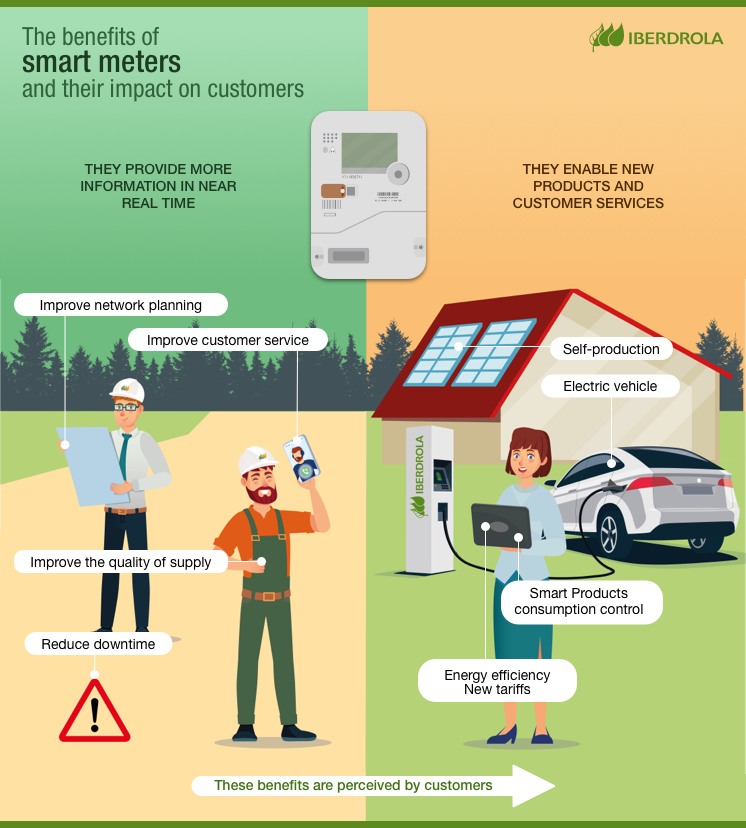
\includegraphics[width=10cm]{Images/Research/Infographic_Smart_Meters_EN.jpg}
    \caption{Uses smart meter\cite{FigureSM}}
    \label{fig:uses_smart_meter}
\end{figure}

\subsection{Types of smart meters}
There are many different types of smart meters. The specific meters are smart current meter, smart gas meter, smart water meter and smart heat meter\cite{DiffSMeters}. There are also combo's of this of course. Now there will be looked at the biggest companies that sell smart meters.

\begin{table}[H]
    \hspace{-2.0cm}
    \begin{tabular}{|p{1.5cm}|p{3.8cm}|p{2.7cm}|p{6cm}|p{2.9cm}|}\hline
        \textbf{Number} & \textbf{Electric meters}\cite{TOP10ELECMET} & \textbf{Gas meters}\cite{TOP10GASMET} & \textbf{Heat meters}\cite{TOP10HEATMET}& \textbf{Water meters}\cite{TOP10WATERMET}\\\hline
        1 & Sensus & Elster & Siemens AG & Anglian water\\\hline
        2 & Landis \+ Gyr & General electric & Danfoss& Itron\\\hline
        3 & Itron Inc. & Itron & Diehl Group& Laison\\\hline
        4 & Sojitz co., Ltd & Landis \+ Gyr & Wassion Group Co. Ltd.&Camwater \\\hline
        5 & Exelon & ABB &  Landis \+ Gyr&WEGoT\\\hline
        6 & NES & Aclara & Itron Inc.&Ameresco\\\hline
        7 & Allete, Inc. & Badget meter & IstaInternational GmbH&Business Stream\\\hline
        8 & Honeywell International& Actatis & Elster Group&Thames Water\\\hline
        9 & Scottish power& Diehl metering& Zenner International GmbH \& Company&United Utilities\\\hline
        10 & Siemens & Krohne & Kamstrup&Global Omnium\\\hline
    \end{tabular}
    \caption{Meter companies}
    \label{tab:Meter_companies}
\end{table}

\subsection{Outputs}
By searching what kind of communication is used by smart meters more connections can be found. It is shown in the list below.

\begin{itemize}
    \item Ethernet\cite{ConnectionsSmartMeter}\cite{ConnectionsSmartMeter2}
    \item Power Line Communication\cite{ConnectionsSmartMeter}\cite{ConnectionsSmartMeter2}
    \item Meter bus\cite{ConnectionsSmartMeter}
    \item Digital Subscriber Line \cite{ConnectionsSmartMeter2}
\end{itemize}


% \section{Router}
% main question: How will the modular router be made?

% \section{Sub-questions}
% \begin{itemize}
%     \item How big should the router be?
%     \item What is the price that can be charged for the completed router?
%     \item Who would use this product?
%     \item How can the esp32 be used for the router?\cite{esp32_monitoring}
%     \item how to flash an ESP32 board\cite{FlashingESP32}
% \end{itemize}

% \subsection{Methodology}
% To answer the main question the sub-questions need to be answered. To answer the sub-question it is important to explain the methods used. The methods are given below. The sources for the research will mainly be searched with the google scholar search engine and Elsevier. 

% \subquestion{1}{How big should the router be?}{2}
% This question could be answered the best for how big routers are\\\\
% \subquestion{2}{What is the price that can be charged for the completed router?}{2}
% This will be done by looking at similar products that aim to have the same use.\\\\
% \subquestion{3}{Who would use this product?}{2}
% This can be done by asking people via a quiz or by searching for marketing stuff\\\\
% \subquestion{4}{How can the esp32 be used for the router?}{2}
% This is researched by searching for what the esp32 had been used before\\\\
% \subquestion{5}{How to flash the esp32 board?}{2}
% Looking at how people flash the esp32 and what the options are.
% \\\\


% \subsection{Size of the router}
% In order to solve the size of the router it needs to compare different routers and see what can fit in a fuse box. 

% \subsection{Price router}
% This will be researched by looking at other comparable routers

% \subsection{Users}
% What kind of people would use the product.

% \subsection{The esp32}
% It is a microcontroller

% \subsection{Flashing the esp32}
% To flash the esp32 there are two general options. Number one is that a devkit is used and places on top of the PCB or the esp32 will be placed directly in order to flash it from one PCB. This will be cheaper and make the PCB smaller.
